\begin{figure}[H]
\centering
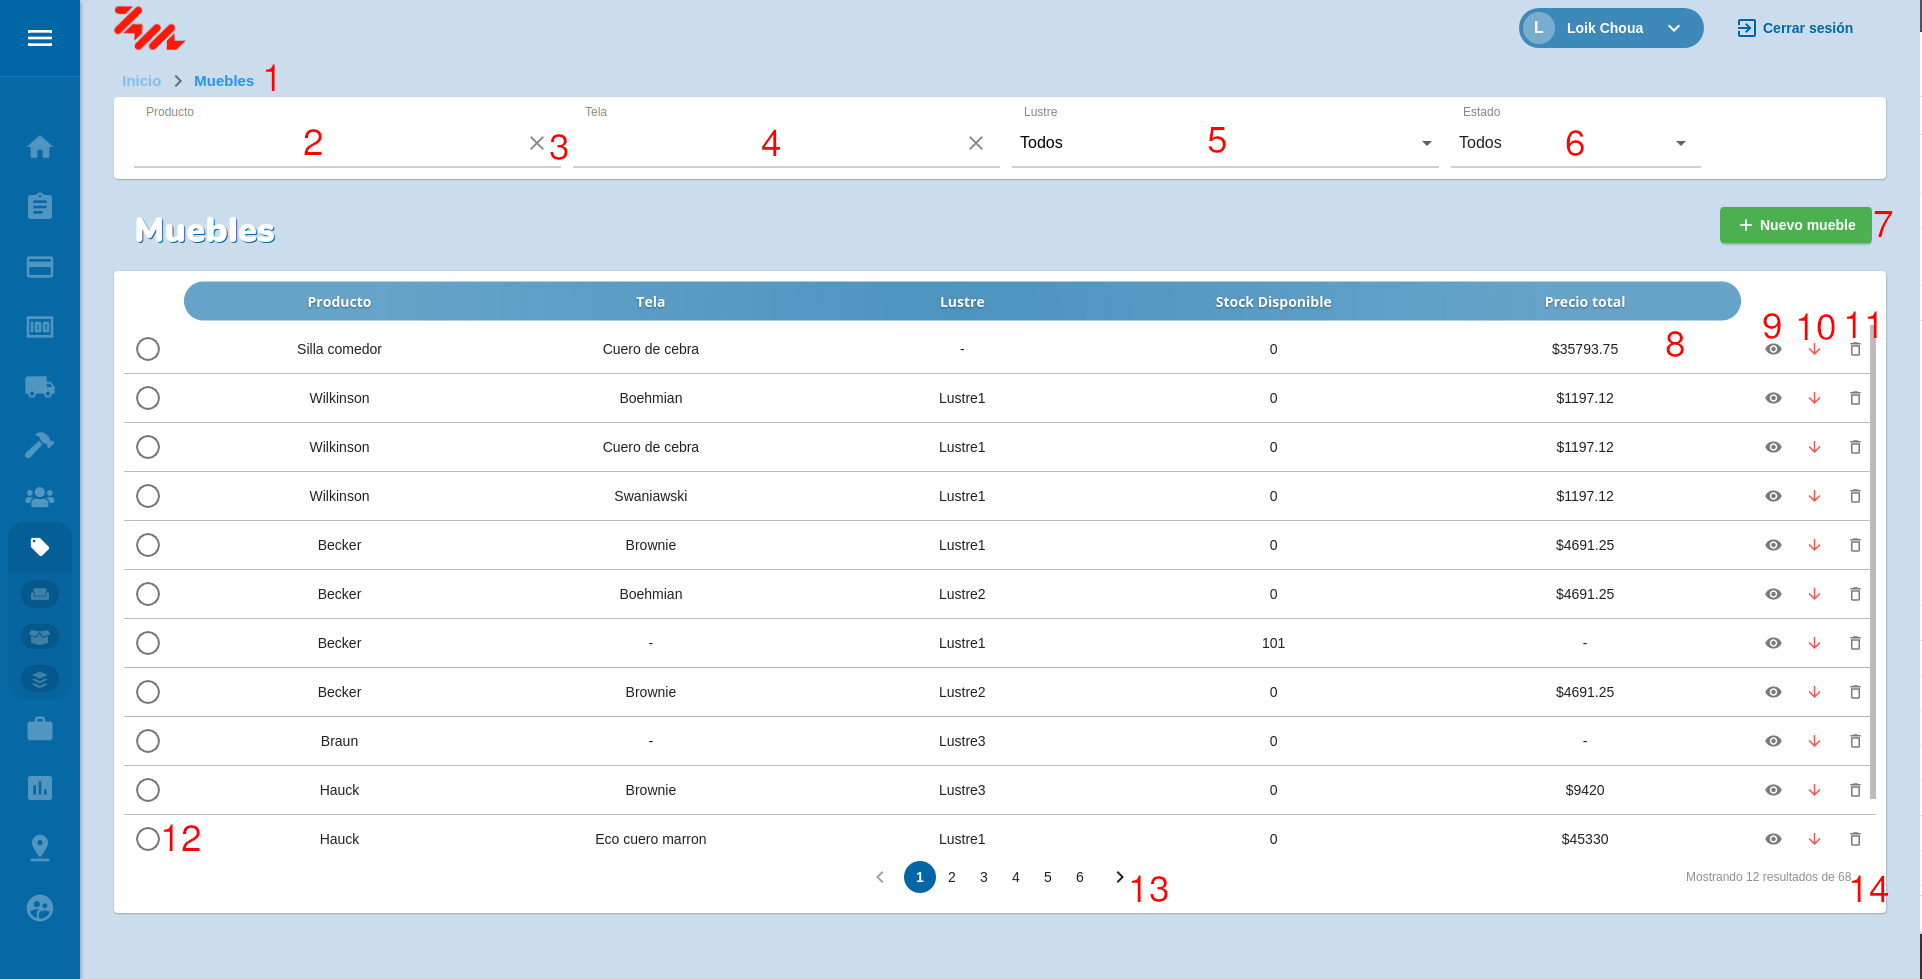
\includegraphics[width=\textwidth,height=\textheight,keepaspectratio]{Escenarios/AD-48-00}
\caption{Escenario - AD-48-00}
\label{fig:AD-48-00}
\end{figure}

Este escenario muestra toda la información referida a los muebles, junto con las acciones disponibles.
El botón \textbf{AD-48-01} permite navegar al escenario \textbf{AD-02-00}. El campo \textbf{AD-48-02} permite ingresar un producto para filtrar los muebles por producto, el campo cuenta con el botón \textbf{AD-48-03} que permite borrar el texto ingresado en el campo. El campo \textbf{AD-48-04} permite al usuario buscar muebles que utilizan una determinada tela. La lista desplegable \textbf{AD-48-05} permite filtrar con un lustre determinado. La lista desplegable \textbf{AD-48-06} permite al usuario filtrar por los estados en los cuales puede encontrarse el mueble.
El botón \textbf{AD-48-07} permite al usuario crear un nuevo mueble y navega al escenario \textbf{AD-49-00}.
El botón \textbf{AD-48-12} permite al usuario seleccionar uno o más muebles del resultado de la búsqueda. Si existen muebles seleccionados se mostrarán botones con las opción de borrar o activar/desactivar según corresponda. El campo \textbf{AD-48-08} muestra la información relacionada a los muebles especificando su código, el producto, tela y lustre que utiliza, stock disponible y precio total del mueble. El botón \textbf{AD-48-09} permite navegar al escenario \textbf{AD-50-00} para ver el mueble, el botón \textbf{AD-48-10} permite al usuario dar de alta/baja un mueble y el botón \textbf{AD-48-11} permite al usuario borrar el mueble. 
En \textbf{AD-48-13} se mostrarán las páginas de resultado, pudiendo cambiar de página. En \textbf{AD-48-14} se mostrará cuántos resultados se están visualizando y el total.
\clearpage
